\section{Abridged 2015-08-12 Product Manager Interview}

\begin{figure}[h]
\centering
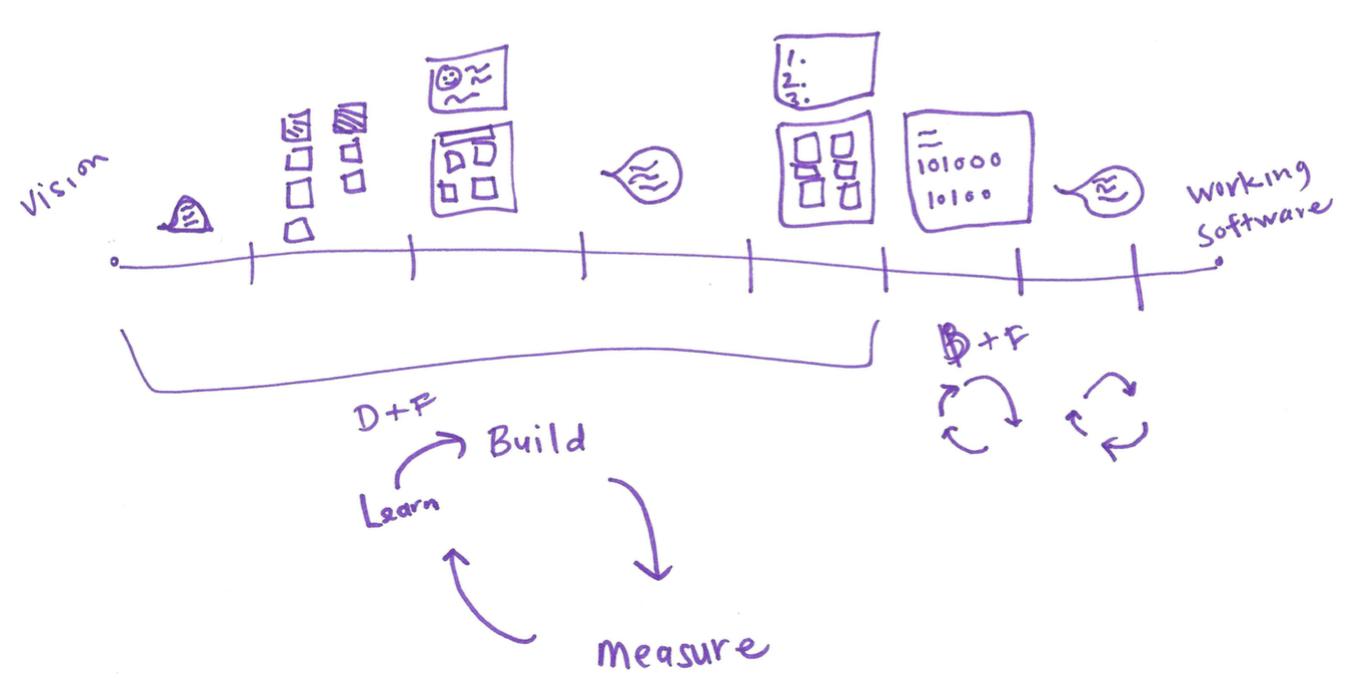
\includegraphics[width=6.5in]{interviews/drawings/2015_08_12_pm.png}
\caption{\quotes{2015-08-12 Product Manager's drawing of software development process}}
\label{2015_08_12_pm}
\end{figure}


\textbf{Todd:} If you're open to it, could you, on that sheet of paper, draw out how you view the way we build software? This is completely open-ended. There's no wrong answers. And just take a stab at it.  0:00:21

\textbf{Interviewee:} So I'm drawing a line, it's like product on a continuum. We're gonna have vision here. We're gonna have working. Can you tell I'm a PM coz I'm writing in lines, boxes can't do? 0:00:45

\textbf{Todd:} I love it.  0:00:46

\textbf{Interviewee:} So let's see here. So let's do a couple of lines here. Alright, so let's say, each of these represents two weeks.  So we'll say that the first point, so how we build it at pivotal is that what you asked?  0:01:17

\textbf{Todd:} Yes.  0:01:18

\textbf{Interviewee:} So it starts with having clients.  0:01:20

\textbf{Todd:} How would you build it too?  0:01:21

\textbf{Interviewee:} Yeah, yeah. Totally. The reason I asked about Pivotal is 'cause we're doing consulting. So if you're thinking of product as a continuum, our clients come in in all these different ways of where they the insert. But it starts with a conversation, kind of like a qualifying conversation of like, 'hey, what do you wanna build?', and like 'what's the fidelity of your idea?' And from there, we have a good understanding of if they're at a stage where they can build something, or if they maybe really need to think about it further.  But once we realize ok, they're ready for Pivotal , we'll start with a Discovery and Framing and not every project gets Discovery and Framings, but in the LA office, a lot of them do.  We're trying to get like most projects getting some a semblance of Discovery and Framing.   0:02:04

\textbf{Todd:} When would you not do one?  0:02:07

\textbf{Interviewee:} So we won't do one... I think we can make the case really for all projects could do with a little bit of DNF right? So even if you're like, I know where to build from. So with FYI rather, but for a PM, I'm thinking, okay my role is to help the client understand who are we building for and then what we are building and when? So for the, who are we building for, I think all clients.  It'd be great if we could do some user research with them even if they are like, we did all these user research just to do a quick gut check, like hey this makes sense, that'll be great.   0:02:42

\textbf{Interviewee:} But I think a lot of the times when we don't do them, it tends to be convincing the client or if there's a budget concern.  So they have enough of a fidelity of understanding who their target user is and who the secondary users are and have a persona and are focused on stuff like kinda key factors like, ok, if you're saying you want to build an app for the millennials and for college-age students and for the ages 25-35, that's pretty vague.  We do get that a lot, but we're saying, ‘ok, it's for millennials, so what gender are we going for?' Or is it, ‘what are their behaviors like?'  There's a lot of questions that we can ask on this conversation. and these qualifying calls to say, to kind of fish out, to think if they are ready to work with Pivotal, or if they have enough information for DNF or not. So, does that answer?  I guess that was a very specific answer.  0:03:44

\textbf{Todd:} That was great.  0:03:46

\textbf{Todd:} I interrupted your flow.  0:03:48

\textbf{Interviewee:} No, no, this is fine.  So I'm of the opinion that I would love it if we could have some sort of research with all of our clients and users. Typically when we do a DNF, Discovery and Framing, we do that for 4 weeks on average, sometimes it's up to 6 weeks depending on how many users they have and how many people they want us to focus on.  But we typically really try to work on 2 to 3 target users being 1 primary user and maybe 2 users of the system that kind of insert in their day.  And then we've done a 2 week of design first or Discovery and Framing but really it's just 'let's talk to some users and validate some ideas.' But the whole goal of this Discovery and Framing process is to do a couple of weeks of talking to users, of about 2 weeks and that's when we're doing some of those exploratory interviews, kinda turn it into elicit narratives to understand what their behaviors and what their days are like.   0:04:51

\textbf{Interviewee:} And then from there, we can isolate what are some of their pain points and what are some of the frictions and inefficiencies and how are they capturing data and what are the tools that they use and who are the people they're talking to.  From there, I guess one thing I didn't mention which is important is to say, what are the product goals that our clients have?  And what are some of the assumptions that they have about their products?  About their users where their products can help solve their needs.  We go into these user research thing like, alright, here are some assumptions, hypothesis that we have, let's test them. Out of that output of user research is that we have this, we do some synthesis and analysis of all of the things they're talking about.  We record the things that we saw, so if they're in a cubicle and they have tons of printed out papers because what they do is they get stuff by mail and then they have to scan it in.  Those are the things that we're seeing that are part of their day that can affect them.   0:05:54

\textbf{Interviewee:} What did we hear, like things that they're telling us about their day, and things like we felt that they're telling us. But maybe there are some subtext and some nuance there saying everything's great but their faces are really strained and you can tell they're really frustrated and their posture has changed when they're talking about certain subjects. Kind of taking all of the things that recording from our user sessions and then coding it by what we saw, what we heard, what we felt and then finding themes. What are users talking about? Usually when we do research, we try to do 3 to 5 users, so that way we have a good cross-sample and in case there's any extreme people that we meet, it kind of helps us give a better analysis, better data sample. So we'll kind of call all the information that we have and we'll go to them, too.  So we'll go to their cubicles or wherever their workspaces are. So we want to get a sense of their environment. Cause there's so much contextual information there that you can't get just from having a phone call with someone.  0:07:02

\textbf{Todd:} Yes.  0:07:03

\textbf{Interviewee:} So, then, that's usually about a couple of weeks doing some researching.  As we're doing the researching, we're capturing all of our information on notepads and then we're doing what we call infinity mapping, affinity mapping.  We'll get one of those big phone cork white boards and we'll take a listen to the recordings of when we're doing user research or if we can't record just looking at our notes ‘coz our notes are like, you're almost writing verbatim what people are saying.  Coz you don't want to put all your analysis in there at this point, you just want to get them to talk and get it all in, and then we'll take each kind of idea and we'll put it on a post-it note and we'll have a bunch of post-it notes around and they'll be coded by what we saw, what we heard, what we felt, and then we'll start seeing themes around this post-it notes.   0:07:54

\textbf{Interviewee:} So there's this one user that said there is a lot of things around education and tools and timeline and whatever it is.  Then we started noticing trends, so we'll start taking those nuggets and we put them across this themes and then we'll do that to all our users; and then from there, we'll do another round of synthesis and the ideas are going to keep condensing.  So then we have a synthesis of all the people we talk to and what the overlaps are and the themes of what their day is like, and the behaviors they drawn during that day.  And then after that, we'll map out their day, like what are the tasks that they're doing, and then map out from the tasks all those insights rather not insights but nuggets of what we heard from them, that we kind of collectively called down and condensed and we'll put those against the tasks.    0:08:43

\textbf{Interviewee:} So when they need to schedule a user for an event, these are all the things they said about it, or these are the things we saw and the things that we felt.  So then what's cool about that is we do that for every target user and you can map them out.  So you say 'here are three target users, here are their days and here are all the intersections of their days'.   So you can tell visually, 'oh, you know what, when this person does something, you notice the next thing, like, these two people are affected.' And then you can start isolating pain points and inefficiencies and you get these really nice overlay of what the system, not the digital system but just the users in the workplace and what their days look like.  So when I'm mapping out the process, I'm thinking of conversations, that's a little talk bubble.  0:09:43

\textbf{Todd:} Ok, I like it.  0:09:44

\textbf{Interviewee:} And then I'm having doing some synthesis. Someone do a little post-it map.  0:09:51

\textbf{Todd:} Ooh, I see the post-its.  0:09:53

\textbf{Interviewee:} There you go.  And then from that, we say, 'ok, based on our research, this is what we say a persona or what this user looks like.'  We think of 'what do they need? What are the tasks in their day and what do we need.'  So we pull out insights from that. Like, this user really has trouble communicating with the other people on this team because they don't have the right communication tools setup or whatever that is. They need a better communication system.  Once we have these needs, and bits and insights of who they are and what they need, then we can say, "all right, how can our products solve these needs?" So then we say, 'we have some product ideas based on what their needs are, let's validate them.'   0:10:55

\textbf{Interviewee:} Then we'll go back and talk to the users. We'll drop some wireframes and say, "all right, based on what you guys had said, we feel that here's a quick prototype, clickable prototype" And we'll use invision.  We'll say, "Why don't you click around? What do you think about these things?" we'll do some user testing there.  And then from that information, we'll further validate or dis-validate our product ideas and we'll do another product evolution but kind of the output of this 4 week on average DNF cycle as that you'll have Wireframes and then you'll have some personas. You'll know who your end user is.  You'll have empathy drawn for your end user which is the whole goal. You'll have a problem that's been framed and validated.   0:11:38

\textbf{Interviewee:} So that way, it really de-risks development cause it's pretty great to come in to development and we know that when we're making product decisions, we can go back to this research.  We're like, "oh, if we're going to do this or this, like, what do they actually need? Like what was that they talked about that really indicated this is the right approach?" It also helps us speak a language that our users speak.  Which is really important for the development team but all the other stakeholders involved in the process.  0:12:05

\textbf{Interviewee:} Words are everything, right? So we want people to be kind of on the same communication levels of talking how their users would talk, so that way it helps us draw all that empathy throughout the entire development process coz you still need to draw on that, you know 6 weeks, 3 months, however long into the development cycle until you're releasing. Right to be able to have that insight of what they want. I think the cycle is... Let's just say that you've done some analysis and you've done some wireframing, and then after that, we'll talk to users again.  After that, we'll do another set of wireframes. We'll also do some persona mapping here as well as making these wireframes.  And then after we do that, we will create a feature list.  0:13:13

\textbf{Todd:} Yes.  0:13:14

\textbf{Interviewee:} So, we'll say, like, we're not gonna…  Like, what could the next you know 2 to 3 kind of epic areas. We'll say, let's give some insights here.  Like, maybe, we have 3 insights and 3 needs.  Let's do 3 feature ideas and how do these feature ideas map these needs?  So we write these feature ideas and we'll say, down in the documents and user needs this and we'll help them achieve their goals.  Business needs this and this will help them achieve their goals.  We're always aligning user business needs throughout the entire process. So then when we get into development, we'll just make a little terminal, I wish I had multiple colors.  0:14:00

\textbf{Todd:} Next time, you'll have to bring your can.  0:14:03

\textbf{Interviewee:} So, when you're getting into the computer, when you're getting into development, you're able to have a backlog that's been built.  You have the first couple of weeks of features.   0:14:17

\textbf{Todd:} Yes.  0:14:18

\textbf{Interviewee:} You have some ideas and you start building and then once you release something, which could be in a week or could be a couple of weeks depending on what you're doing.  But once you get into the first bit of business value working software, then you can go and you could talk to your users again and then you learn from them and then you continue on.  So at that point, what you're doing is you're building something and then you're measuring it.    0:14:45

\textbf{Todd:} Yes.   0:14:46

\textbf{Interviewee:} And then you're learning from it right?   0:14:48

\textbf{Todd:} Uh-huh. Yes.  0:14:50

\textbf{Interviewee:} And then you're going back to building, right? So that's what we're doing for this whole process. So the feedback loop is really important.  I think, when I'm thinking about the extent, like the depth of all these research, you don't need to have a DNF to do any of these research, right?  You don't have to sell that in, you can do...  So the training that our designers and our PMs have, and now we're trying to have our developers be exposed to it, as well.  To say, ‘ok, developer, you get a client project. Development starts tomorrow, you can still talk to some users.  You can still setup user testing.'  And you can do that throughout the entire process.  So it's almost like this whole upfront part, with like the DNF.  You're making little DNFs through it, right?  So whoops, it's really you're taking this and you're kind of doing like DNF cycle.   0:15:42

\textbf{Todd:} Yeah.   0:15:43

\textbf{Interviewee:} Whoops, and you're doing that here, and then you're going to do it again. So, like each week, you might be bi-weekly.   And that is ideal, right?  But sometimes you don't get the users?  So there's a lot of, kind of…  You have to be pretty scrappy with how you do this sometimes, you don't just get this nice set of users at your disposal, you know; but it's so important and I think that's something we do a good job with is convincing our clients, like, we wanna de-risk this for you so this is how we can do it.  I mean go, it makes sense.  It's very practical stuff.  It's not rocket science honestly.   0:16:20
